\documentclass[12pt,letterpaper]{exam}
\usepackage[lmargin=1in,rmargin=1in,tmargin=1in,bmargin=1in]{geometry}
\usepackage{../style/exams}

% -------------------
% Course & Exam Information
% -------------------
\newcommand{\course}{MATH 111I: Exam 1}
\newcommand{\term}{Spring --- 2025}
\newcommand{\examdate}{02/13/2025}
\newcommand{\timelimit}{75 Minutes}

\setbool{hideans}{true} % Student: True; Instructor: False


% -------------------
% Content
% -------------------
\begin{document}

\examtitle
\instructions{Write your name on the appropriate line on the exam cover sheet. This exam contains \numpages\ pages (including this cover page) and \numquestions\ questions. Check that you have every page of the exam. Answer the questions in the spaces provided on the question sheets. Be sure to answer every part of each question and show all your work. If you run out of room for an answer, continue on the back of the page --- being sure to indicate the problem number.} 
\scores
\bottomline
\newpage


% -------------------
% Questions
% -------------------
\begin{questions}

% Question 1
\question[5] Find an expression that gives the price of an item that costs $P$~dollars after it has been discounted by 40\%. \pspace

{\itshape After the item has been discounted by 60\%, only 40\% of its price remains. We know to find a percentage of a number, we multiply the number by the percentage as a decimal. But then the cost of the item is $0.60 P$. Alternatively, we know the 40\% discount is given by $0.40P$. We then need to remove this price from the price of the item, $P$. But then the cost of the item is $P - 0.40P$. Observe these are the same because\dots
	\[
	P - 0.40P= P(1 - 0.40)= P \cdot 0.60= 0.60P
	\]
} \pvspace{3.8cm}



% Question 2
\question[5] The CEO of EducateU, an education research non-profit, gave the following statement:

{\itshape We here at EducateU are revolutionizing education. Because of our tireless efforts for years, we have found an equation for intelligence---to predict future success. We have discovered that the future income of an average student with IQ $I$ is nearly perfectly predicted by\dots
	\[
	I^{2/3} - \dfrac{14}{I} + 20
	\]
}
Explain what is mathematically wrong about the CEO's statement. \pvspace{1.83cm}

{\itshape The given `equation' is not an equation; it is a mathematical expression because there is no equality, inequality, etc.}



% Question 3
\newpage
\question[15] Find the average rate of change of $f(x)= 3x^2 + 2$ on the interval $[-1, 2]$. \pspace

{\itshape \tsol We know the average rate of change for a function is the slope of the line through the graph of the function at the endpoints of the interval, i.e. $\dfrac{f(b) - f(a)}{b - a}$. We have $a= -1$ and $b= 2$, so that\dots
	\[
	\begin{aligned}
	f(2)&= 3(2^2) + 2= 3(4) + 2= 12 + 2= 14 \\[0.3cm]
	f(-1)&= 3(-1)^2 + 2= 3(1) + 2= 3 + 2= 5
	\end{aligned}
	\]
Therefore, the average rate of change is\dots
	\[
	\text{Avg. ROC}= \dfrac{f(2) - f(-1)}{2 - (-1)}= \dfrac{14 - 5}{2 + 1}= \dfrac{9}{3}= 3
	\]
}



% Question 4
\newpage
\question[15] Consider the relation $f(x)$ plotted below. 
	\[
	\fbox{
	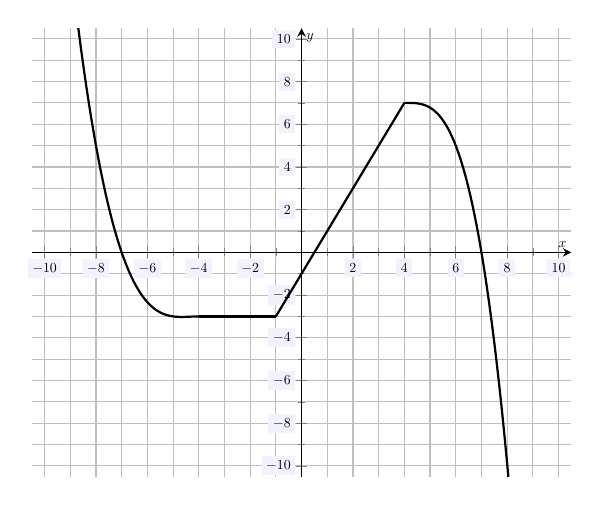
\begin{tikzpicture}[scale=1,every node/.style={scale=0.5}]
	\begin{axis}[
	grid=both,
	axis lines=middle,
	ticklabel style= {fill= blue!5!white},
	xmin= -10.5, xmax=10.5,
	ymin= -10.5, ymax=10.5,
	xtick= {-10,-8,...,10},
	ytick= {-10,-8,...,10},
	minor tick = {-10,-9,...,10},
	xlabel= \(x\), ylabel= \(y\)
	]
	\addplot[thick, samples=150, smooth, domain= -10.5:-4] {-(5 + (8*(x + 2))/3 + (7*(x+2)^2)/6 + (x+2)^3/6)};
	\addplot[thick, samples=5, smooth, domain= -4:-1] {-3};
	\addplot[thick, samples=5, smooth, domain= -1:4] {-(5 - 2*(x+2))};
	\addplot[thick, samples=100, smooth, domain= 4:10.5] {-(-69 + (92*(x+2))/3 - (91*(x+2)^2)/18 + (5*(x+2)^3)/18)};
	
	\end{axis}
	\end{tikzpicture}
	}
	\]

\begin{enumerate}[(a)]
\item Determine whether $f(x)$ is a function. Be sure to justify your answer. \pvspace{0.7cm}

{\itshape Yes, $f(x)$ is a function because it passes the vertical line test, i.e. every vertical line intersects the graph at most once.} \pvspace{0.7cm}

\item Determine the $x$-intercepts for $f(x)$. \pvspace{0.6cm}

{\itshape The $x$-intercepts are the points where $f(x)$ intersects the $x$-axis. These are $x= -7, 0.5, 7$.} \pvspace{0.6cm}

\item Determine the $y$-intercepts for $f(x)$. \pvspace{0.7cm}

{\itshape The $y$-intercepts are the points where $f(x)$ intersects the $y$-axis. This is $y= -1$.} \pvspace{0.7cm}

\item Find $f(4)$. \pvspace{0.7cm}

{\itshape Examining the graph, we see that $(4, 7)$ is on the graph. Therefore, $f(4)= 7$.} \pvspace{0.7cm}

\item Find the solutions to $f(x)= 5$. \pvspace{0.7cm}

{\itshape If $f(x)= 5$, then $(x, 5)$ is a point on the graph, i.e. the graph intersects the line $y= 5$. Examining the plot, we see the solutions are $x= -8, 3, 6$.}
\end{enumerate}



% Question 5
\newpage
\question[15] Consider the system of linear equations given below:
	\[
	\begin{cases}
	3x + 2y= 7 \\
	6x - y= -11
	\end{cases}
	\]

\begin{enumerate}[(a)]
\item Without explicitly solving the system of equations, determine if there is a solution to the system of equations. Be sure to fully justify your answer. \pspace

{\scriptsize \itshape We know a system of two linear equations has a solution if and only if the lines intersect. Observe that\dots
	\[
	\begin{aligned}
	3x + 2y&= 7 \qquad& 6x - y&= -11 \\
	2y= -3x& + 7 & -y= -6x& - 11 \\
	y= -\frac{3}{2}\, x & + \frac{7}{2} & y= 6x& + 11
	\end{aligned}
	\]
The slope of the first line is $m_1= -\frac{3}{2}$ and the slope of the second line is $m_2= 6$. Because $m_1 \neq m_2$, the lines are not parallel. Because the lines are not parallel, the lines intersect. Therefore, there is a solution to the given system of equations.}

\item Find the solution to the given system of equations. \pspace

{\itshape Using substitution, we solve for $y$ in the second equation to find $y= 6x + 11$. Using this in the first equation, we have\dots
	\[
	7= 3x + 2y= 3x + 2(6x + 11)= 3x + 12x + 22= 15x + 22
	\]
But then $15x + 22= 7$, which implies that $15x= -15$. Therefore, $x= -\frac{15}{15}= -1$. But then $y= 6x + 11= 6(-1) + 11= -6 + 11= 5$. Therefore, the solution is $x= -1$ and $y= 5$, i.e. $(x, y)= (-1, 5)$. \pspace

Alternatively, we can use elimination. Multiplying the second equation by $2$, we have\dots
	\[
	\begin{aligned}
	3x + 2y&= 7 \\
	12x + (-2y)& -22
	\end{aligned}
	\]
Adding these equations, we find $15x= -15$. But then $x= \frac{-15}{15}= -1$. Using the second equation, we have $-11= 6x - y= 6(-1) - y= -6 - y$. But then $-11 + y= -6$, so that $y= 5$. Therefore, $y= 11 - 6= 5$. Therefore, the solution is $x= -1$ and $y= 5$, i.e. $(x, y)= (-1, 5)$.}

\item Verify your solution in (b) to the given system. \pspace

{\itshape We verify that $x= -2$ and $y= 3$ satisfy both of the equations simultaneously:
	\[
	\begin{aligned}
	3x + 2y&= 7 \qquad& 6x - y&= -11 \\
	3(-1) + 2(5)&\stackrel{?}{=} 7 & 6(-1) - 5&\stackrel{?}{=} -11 \\
	-3 + 10&\stackrel{?}{=} 7 & -6 - 5&\stackrel{?}{=} -11 \\
	7&= 7 & -11&= -11
	\end{aligned}
	\]
Therefore, $(x, y)= (-1, 5)$ is a solution.}
\end{enumerate}



% Question 6
\newpage
\question[15] Little Susie hires a tax advisor to not run afoul of the law running her lemonade stand. The advisor finds that the amount of money, $M$, she makes $d$ days from now is given by $M(d)= 16d + 25$.
	\begin{enumerate}[(a)]
	\item Explain why $M(d)$ is a linear function. \pvspace{2.6cm}
	
	{\itshape A linear function has the form $y= mx + b$. We know that $M(d)$ has the form $y= mx + b$ with $y= M$, $x= d$, $m= 16$, and $b= 25$. Therefore, $M(d)$ is linear.} \pvspace{2.6cm}
	
	\item Find and interpret the slope of $M(d)$. \pvspace{2.32cm}
	
	{\itshape We know from (a) that $m= 16$. We know that $m= \frac{\Delta \text{ouput}}{\Delta \text{input}}= \frac{Delta M}{\Delta t}$. But then $m= +16$ has units of money per day. Therefore, Little Susie makes \$16 per day, i.e. she makes \$16 in sales per day.} \pvspace{2.32cm}
	
	\item Find and interpret the $y$-intercept of $M(d)$. \pvspace{2.4cm}
	
	{\itshape We know from (a) that $b= 25$. We know that $b= 20$ is the output when $d= 0$. But then at $d= 0$, the amount of money is $M= 25$. Therefore, Little Susie has already made \$25 running her stand by the time she hires the tax advisor.} \pvspace{2.32cm}
	\end{enumerate} 



% Question 7
\newpage
\question[15] Let $\ell(x)$ be the linear function with slope $-2$ through the point $(-1, 5)$. 
	\begin{enumerate}[(a)]
	\item Find $\ell(x)$. Express your answer in the form $\ell(x)= mx + b$. \pvspace{0.5cm}
	
	{\itshape We know the line has the form $\ell(x)= mx + b$. We are told the slope is $-2$, i.e. $m= -2$. We now that $\ell(x)= -2x + b$. Furthermore, we know that $(-1, 5)$ is on the graph, i.e. $\ell(-1)= 5$. But then\dots
		\[
		\begin{gathered}
		\ell(x)= -2x + b \\
		\ell(-1)= -2(-1) + b \\
		5= 2 + b \\
		b= 3
		\end{gathered}
		\]
	Therefore, $\ell(x)= -2x + 3$ or $\ell(x)= 3 - 2x$.
	} \pvspace{4.55cm}

	\item Find $\ell(4)$. \pvspace{0.5cm}
	
	{\itshape We know that $\ell(x)= -2x + 3$ from (a). But then\dots
		\[
		\ell(4)= -2(4) + 3= -8 + 3= -5
		\]
	}
	\end{enumerate}



% Question 8
\newpage
\question[15] A physicist is examining the effect of finite heat pulses in a metal rod. They find that after the rod is subjected to a finite heat pulse that the temperature increases at a constant rate of 25$^\circ$F per minute. The initial temperature of the rod is 80$^\circ$F. Let $T(m)$ be the temperature of the rod (in $^\circ$F) after $m$~minutes. 
	\begin{enumerate}[(a)]
	\item Explain why $T(m)$ is linear. \pvspace{2cm}
	
	{\itshape A linear function has a constant rate of change. We are told that the temperature of the rod increases at a constant rate of 25$^\circ$F per minute. Therefore, the rate of change of temperature of the rod is constant. This shows that the temperature of the rod is linear in time.} \pvspace{2cm}
	
	\item Find the function $T(m)$. \pvspace{1.95cm}
	
	{\itshape We know the rate of change in the temperature of the rod is $m= 25$. We know also that the initial temperature of the rod was 80$^\circ$F, i.e. the temperature at time $m= 0$ (the $y$-intercept) was 80$^\circ$F. But then $b= 80$. Because $T(m)$ is linear, it has the form $mx + b$. But we know that $m= 25$ and $b= 80$. Therefore, $T(m)= 25m + 80$.} \pvspace{1.95cm}
	
	\item How long until the temperature of the rod is 430$^\circ$F? \pvspace{1cm}
	
	{\itshape If $m$ is a minute from now when the rod was 430$^\circ$, then $T(m)= 430$. But then\dots
		\[
		\begin{gathered}
		T(m)= 430 \\
		25m + 80= 430 \\
		25m= 350 \\
		m= 14
		\end{gathered}
		\]
	Therefore, the temperature of the rod will be 430$^\circ$F in 14~minutes. 
	}
	\end{enumerate}

\end{questions}
\end{document}